\documentclass[11pt,letterpaper]{article}
\usepackage[T1]{fontenc}
\usepackage[utf8]{inputenc}
\usepackage{newtxtext,newtxmath}
\usepackage[margin=0.9in,headheight=15pt,headsep=20pt,footskip=28pt]{geometry}
\usepackage{microtype}
\usepackage{amsmath}
\usepackage{booktabs,tabularx,array,longtable}
\usepackage{graphicx,tikz}
\usetikzlibrary{arrows.meta,positioning,calc}
\usepackage{enumitem}
\usepackage{fancyhdr}
\usepackage{titlesec}
\usepackage{caption}
\usepackage{listings}
\usepackage{needspace}
\usepackage[hidelinks,unicode]{hyperref}
\hypersetup{pdftitle={Zoetrope: A Deadline-Aware Architecture for Continuous Multimodal Perception, Reasoning, and Authorized Action},pdfauthor={Payton Ison},pdfsubject={Conceptual systems research proposal; version 0.1},pdfkeywords={streaming video, multimodal reasoning, temporal memory, real-time agents, evidence freshness}}
\pagestyle{fancy}
\fancyhf{}
\fancyhead[L]{\small\textsc{Zoetrope}}
\fancyhead[R]{\small Research proposal\;\textbullet\;v0.1}
\fancyfoot[C]{\small\thepage}
\renewcommand{\headrulewidth}{0.3pt}
\setlength{\parindent}{1.25em}
\setlength{\parskip}{2.5pt}
\linespread{1.025}
\titleformat{\section}{\large\bfseries}{\thesection}{0.65em}{}
\titleformat{\subsection}{\normalsize\bfseries}{\thesubsection}{0.65em}{}
\titlespacing*{\section}{0pt}{15pt plus 3pt minus 2pt}{7pt}
\titlespacing*{\subsection}{0pt}{11pt plus 2pt minus 2pt}{4pt}
\captionsetup{font=small,labelfont=bf,skip=7pt}
\setlist{itemsep=2pt,topsep=5pt,leftmargin=1.5em}
\emergencystretch=1.5em
\widowpenalty=10000
\clubpenalty=10000
\newcolumntype{Y}{>{\raggedright\arraybackslash}X}
\newcommand{\E}{\mathbb{E}}
\newcommand{\ind}{\mathbf{1}}
\newcommand{\refentry}[1]{\par\begingroup\small\setlength{\parindent}{0pt}\hangindent=1.3em\hangafter=1 #1\par\endgroup\vspace{5pt}}
\lstset{basicstyle=\footnotesize\ttfamily,columns=fullflexible,keepspaces=true,breaklines=true,frame=single,framerule=0.3pt,xleftmargin=3pt,xrightmargin=3pt,aboveskip=9pt,belowskip=9pt,showstringspaces=false}

\begin{document}
\thispagestyle{empty}
\begin{center}
{\small\textsc{Conceptual systems research}\par}
\vspace{10pt}
{\LARGE\bfseries Zoetrope\par}
\vspace{5pt}
{\Large\bfseries A Deadline-Aware Architecture for Continuous\par
Multimodal Perception, Reasoning, and Authorized Action\par}
\vspace{13pt}
{\normalsize Payton Ison\par}
\vspace{5pt}
{\small 15 October 2026\quad\textbullet\quad Version 0.1\par}
\end{center}
\vspace{4pt}
\begin{abstract}
A live visual assistant must do more than describe successive images: it must maintain a coherent account of an evolving situation, allocate reasoning effort before relevant opportunities expire, and distinguish an authorized action from a plausible but outdated suggestion. We propose \emph{Zoetrope}, a model-agnostic architecture for continuous multimodal perception, asynchronous reasoning, and bounded intervention. Its starting configuration samples every other frame of a video stream. Rather than equating this sampling frequency with the frequency or latency of complete reasoning, Zoetrope separates observation ingestion, temporal state maintenance, reasoning admission, and action execution. A versioned evidence store connects claims to timestamped observations; a deadline-aware scheduler allocates deeper inference; and an independent execution gate revalidates permissions and action-critical evidence before an intervention. The design supports both responsive questions and standing requests that require proactive notice or action, while perception continues during response generation. We formalize the distinction between throughput and freshness, specify bounded-memory and overload behavior, and develop a causal evaluation protocol that measures deadline-conditioned correctness, stale-state errors, interruption burden, and resource use. The central hypothesis is that explicit evidence validity and selective reasoning improve useful real-time performance over isolated frame analysis and asynchronous systems without freshness checks. This manuscript presents an architecture, analytical constraints, and an experimental plan; it reports no implementation measurements or benchmark results.
\end{abstract}
\vspace{2pt}
\noindent\textbf{Keywords:} streaming video; multimodal reasoning; temporal state; asynchronous inference; evidence freshness; bounded agency.

\section{Introduction}
A camera can deliver a new image while an AI system is still interpreting an earlier one. During that interval, an object may move, a speaker may retract an instruction, or the opportunity for a useful response may disappear. A system can therefore produce a correct account of the past and still fail as an assistant in the present. Zoetrope addresses this mismatch between continuous observation and computationally expensive reasoning.

Consider an assistant watching a tabletop task. It is asked to track public game state, answer questions about recent moves, and announce a specified event when it occurs. The assistant should continue watching while explaining an earlier move. It should retain uncertainty when a hand obscures a piece, distinguish a prediction from an observed transition, and avoid acting on a board configuration that has already changed. The same requirements arise in a screen-based workflow: recognizing a button is insufficient if the window changes before a proposed click is executed. These are motivating scenarios, not demonstrations of an implemented system.

The initial Zoetrope concept is a multimodal model that analyzes every other video frame using modern reasoning capabilities, with both continuous understanding and the ability to respond or intervene. This paper preserves that configuration as a meaningful baseline and development target. It also asks which parts of the work must occur for every admitted frame. Uniform observation, frequent state updates, and complete deliberative inference are distinct operations. Treating them as identical can spend substantial computation repeatedly explaining an unchanged scene while delaying a consequential event.

Streaming video interaction is already an established research direction. VideoLLM-online develops learning and inference for continuous video dialogue; Dispider separates perception, decision, and reaction; and ThinkStream incrementally reasons over incoming video (Chen et al., 2024; Qian et al., 2025; Liu et al., 2026). Zoetrope does not claim to originate these ideas. Its proposed research contribution is a systems specification that connects asynchronous reasoning to explicit evidence lifetimes, resource admission, and revalidated action commitments. Whether this combination improves performance is an empirical question.

The paper makes three contributions at the proposal level. First, it defines useful real-time operation in terms of causal evidence, task deadlines, and the state on which a response depends, rather than frame rate alone. Second, it specifies an architecture that continues observation during inference and prevents completed inference from silently overwriting newer knowledge. Third, it defines experiments that can separate the benefits of frequent perception, temporal memory, scheduling, and action gating. The intended result is a reproducible research program, not a claim that a new foundation model or generally reliable embodied agent has already been built.

\section{Related work and research positioning}
\subsection{Continuous video interaction}
VideoLLM-online introduces a Learning-In-Video-Stream framework, including a streaming language-modeling objective, conversion of temporal annotations into dialogue, and an optimized inference pipeline (Chen et al., 2024). Dispider makes the separation between ongoing observation and response generation especially explicit: lightweight processing identifies interaction opportunities while an asynchronous component generates a response (Qian et al., 2025). StreamBridge similarly combines compressed memory with a lightweight activation component to adapt offline video models for proactive interaction (Wang et al., 2025). These systems make an unqualified claim that ``continuous watching while responding'' is new untenable.

Zoetrope instead focuses on the lifecycle of a decision after it has been triggered. Which observed facts justified the computation? Which remain valid when it finishes? Has the user's authorization changed? Can a late answer still be offered as historical commentary, even when the corresponding action must be canceled? These are the interfaces the proposed design makes explicit. The distinction is a proposed experimental emphasis, not a verified claim that prior systems lack every comparable mechanism.

\subsection{Incremental reasoning, memory, and selective observation}
ThinkStream's Watch--Think--Speak formulation updates reasoning as observations arrive and uses reasoning-compressed memory to preserve context while reducing retained visual material (Liu et al., 2026). StreamAgent anticipates task-relevant temporal intervals and spatial regions and maintains a hierarchical streaming cache (Yang et al., 2025). VideoBrain learns adaptive frame acquisition for long-video understanding, illustrating that selecting evidence can itself be part of the reasoning process (Zou et al., 2026). An offline sampler that can inspect an entire recording, however, is not automatically a causal live-stream policy.

Zoetrope uses these directions as foundations. It proposes a bounded hybrid store containing recent visual evidence, structured current-state claims, and selected historical events. Unlike a memory composed solely of generated summaries, each actionable claim retains explicit evidence references and a validity status. This is an architectural choice to be tested against simpler summaries, not a claim that symbolic memory is always more accurate or efficient.

\subsection{Multimodal input and online evaluation}
Qwen2.5-Omni describes block-wise multimodal processing, time-aligned audio--video representation, and separate text-reasoning and speech-generation components (Xu et al., 2025). It provides a relevant model-level example of synchronized modalities and streaming outputs. Zoetrope remains agnostic about the underlying model and does not assume that every backend exposes equivalent streaming, caching, or cancellation capabilities.

StreamingBench evaluates visual, multimodal, and contextual understanding at timestamps within video. Much of its evaluation uses video prefixes rather than continuously running wall-clock systems (Lin et al., 2024). OVO-Bench explicitly considers past events, current understanding, and waiting for sufficient evidence before responding (Li et al., 2025). OVO-S-Bench extends timestamped evaluation to spatial reasoning (Li et al., 2026). These benchmarks supply useful semantic tasks, but deployed latency, permission changes, and actual side effects require additional system-level tests.

\subsection{Freshness, calibration, and agent security}
Age of information distinguishes the freshness of a received update from communication throughput or the duration of its delivery (Yates et al., 2020). Zoetrope adapts this perspective to individual decision dependencies rather than using one timestamp for an entire scene. Probability calibration is also relevant: a confidence value should not be interpreted as a correctness probability merely because a model emits it (Guo et al., 2017).

Image Hijacks demonstrates that visual inputs can manipulate a vision-language model, while AgentDojo evaluates tool-using agents exposed to untrusted data (Bailey et al., 2023; Debenedetti et al., 2024). CaMeL investigates separating trusted control from untrusted data and enforcing capability-based constraints (Debenedetti et al., 2025). Zoetrope adopts independent execution checks as a design principle, without claiming to inherit another system's security guarantees or to solve prompt injection.

\section{Problem formulation}
\subsection{Streams, observations, and causal availability}
Let a session contain video frames $V=\{(x_i,t_i)\}$, audio segments $A=\{(a_k,s_k,e_k)\}$, authenticated user instructions $G$, and tool observations $T$. A video timestamp $t_i$ identifies capture time; an audio interval $[s_k,e_k]$ identifies the sound represented. Each item also has an arrival time $r_i$ on the coordinator's monotonic clock. The distinction matters because capture, transport, decoding, and transcription can introduce different delays.

At wall-clock time $t$, the system may use only observations that have actually arrived by $t$. An output policy is causal when
\begin{equation}
 y_t = \pi\bigl(\mathcal{O}_{\mathrm{available}}(t),G_{\leq t},T_{\leq t},M_t\bigr),
 \label{eq:causal}
\end{equation}
where $M_t$ is memory derived from previously available information. A historical clip may be revisited if retained, but an unreceived future frame may not be consulted. Predictions are allowed; presenting their outcomes as already observed is not. Evaluation must enforce this constraint for auxiliary inputs as well as images: subtitles, transcripts, event labels, and preprocessing caches can otherwise leak future information.

A standing instruction, such as ``tell me when the third token enters the tray,'' defines an ongoing task. A reactive question requests an answer at a particular time. Both are represented as task records containing their scope, success conditions, communication preferences, and any authorized actions. The system is not permitted to derive new authority from text or speech encountered in the scene.

\Needspace{9\baselineskip}
\subsection{A working state, not an omniscient world model}
The working state is
\begin{equation}
 S_t=(O_t,R_t,E_t,H_t,G_t,U_t,v_t),
 \label{eq:state}
\end{equation}
where $O_t$ contains tracked entities, $R_t$ spatial and temporal relations, $E_t$ event records, $H_t$ hypotheses, $G_t$ active tasks, $U_t$ uncertainty and visibility information, and $v_t$ a monotonically increasing commit version. This representation is an operational belief state. It is not a claim that the system possesses a complete causal model of the environment.

Each claim distinguishes observation from interpretation. ``A red token is visible in region B'' is different from ``the player probably intends to move it.'' A predicted event carries an unresolved status until subsequent evidence confirms or rejects it. An object that becomes occluded may remain a tracked hypothesis, but the last observed position is not automatically its present position. Entity identities can be unresolved or branched instead of being forcibly merged.

\subsection{Useful output and decision windows}
For an event or request $j$, let $t_j^\star$ be the earliest time at which the permitted evidence is sufficient for the required response. Let $d_j\geq t_j^\star$ be the last useful response time. The interval $[t_j^\star,d_j]$ is a task-specific decision window. In evaluation, both boundaries are fixed on the shared source or replay clock, not reset when a slow backend receives or notices the evidence. Input delay therefore consumes the available window. A historical explanation may have a long window; a notification about a transient on-screen state may have a short one.

A useful output must be semantically correct, supported by the available evidence, permitted by current policy, and delivered within its decision window. These conditions are distinct. Fast but premature guessing fails; an accurate instruction delivered after the opportunity has passed also fails. Actions require an additional check that their environmental preconditions still hold at commitment. For tasks with ambiguous evidence onset, evaluators should annotate an interval of acceptable onset rather than invent a falsely precise timestamp.

\section{Zoetrope architecture}
\subsection{Overview and execution boundaries}
Zoetrope has four continuously cooperating paths: observation and perception, state maintenance, reasoning, and output execution. Figure~\ref{fig:architecture} shows the main dataflow. The coordinator owns state commits, task scheduling, and permissions. Perception and reasoning workers produce proposals; they do not possess unrestricted authority to mutate external resources. An execution gate mediates both tool actions and user-facing interruptions.

\begin{figure}[htbp]
\centering
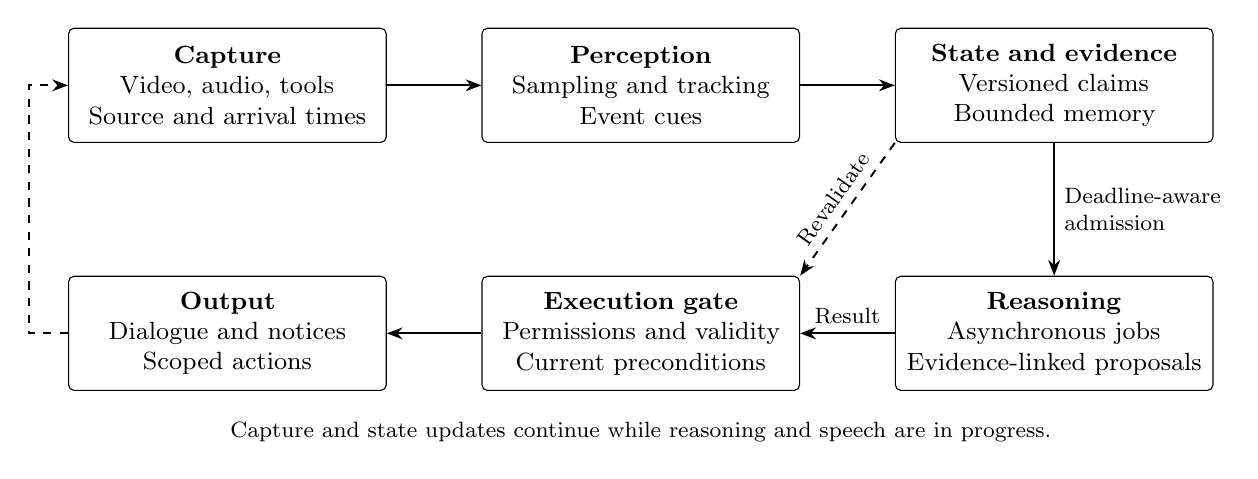
\begin{tikzpicture}[box/.style={draw,rounded corners=2pt,align=center,minimum height=1.45cm,text width=3.8cm,font=\small},flow/.style={-{Stealth[length=2mm]},line width=0.7pt},feedback/.style={flow,dashed}]
\node[box] (capture) at (0,3.15) {\textbf{Capture}\\Video, audio, tools\\Source and arrival times};
\node[box] (perception) at (5.25,3.15) {\textbf{Perception}\\Sampling and tracking\\Event cues};
\node[box] (state) at (10.5,3.15) {\textbf{State and evidence}\\Versioned claims\\Bounded memory};
\node[box] (outputs) at (0,0) {\textbf{Output}\\Dialogue and notices\\Scoped actions};
\node[box] (gate) at (5.25,0) {\textbf{Execution gate}\\Permissions and validity\\Current preconditions};
\node[box] (reason) at (10.5,0) {\textbf{Reasoning}\\Asynchronous jobs\\Evidence-linked proposals};
\draw[flow] (capture) -- (perception);
\draw[flow] (perception) -- (state);
\draw[flow] (state) -- node[right,font=\footnotesize,align=left]{Deadline-aware\\admission} (reason);
\draw[flow] (reason) -- node[above,font=\footnotesize]{Result} (gate);
\draw[flow] (gate) -- (outputs);
\draw[feedback] (state.south west) -- node[above,sloped,font=\footnotesize,pos=0.5]{Revalidate} (gate.north east);
\draw[feedback] (outputs.west) -- ++(-0.5,0) |- (capture.west);
\node[font=\footnotesize,align=center] at (5.25,-1.25) {Capture and state updates continue while reasoning and speech are in progress.};
\end{tikzpicture}
\caption{Proposed Zoetrope dataflow. Solid arrows show the main processing path; dashed arrows show revalidation and environmental feedback. Validated state-update proposals return through the coordinator, which serializes commits. The figure specifies interfaces, not measured timing or a particular neural architecture.}
\label{fig:architecture}
\end{figure}

Decoupling is logical before it is physical. Separate threads that contend for the same fully occupied accelerator may still block one another in practice. The implementation must therefore reserve or prioritize enough processing capacity for ingestion and cheap state updates, and measure contention under load. Distributed workers add transport and ordering complexity; they are an optional deployment, not a prerequisite for the concept.

\subsection{Observation and the every-other-frame configuration}
For a source frame rate $f_v$ and fixed stride $k$, the nominal sampled rate is
\begin{equation}
 f_s=\frac{f_v}{k}.
 \label{eq:sampling}
\end{equation}
The original proposal corresponds to $k=2$. At 30 frames per second, this admits 15 sampled frames per second, separated nominally by about 66.7 milliseconds. That spacing is neither a guarantee that each frame is delivered on time nor a requirement that every full reasoning job finish within 66.7 milliseconds. Variable frame rates and dropped packets require timestamp-based accounting rather than an assumed cadence.

We define two explicit instantiations. \emph{Dense Zoetrope} schedules a complete reasoning request for each sampled frame, optionally with a causal recent window and prior state. It preserves the literal every-other-frame reasoning hypothesis. \emph{Adaptive Zoetrope} admits the same sampled observations to fast perception but invokes deeper reasoning selectively. A result for the adaptive system must not be advertised as proof that dense reasoning has reached the same rate. Reports must state capture rate, admitted observation rate, model-visible frame rate, reasoning-request rate, and useful decision rate separately.

Fast perception may include visual embeddings, task-specific object tracking, region changes, and short-window temporal features. Audio contributes speech boundaries and sound-event cues. These are candidate components, not a prescribed dependency stack. Motion cannot be reconstructed reliably by treating every image as unrelated to its neighbors; temporal order and elapsed time remain part of the evidence. A low-change scene also cannot be assumed irrelevant: a small counter change or a spoken correction may be decisive.

Fixed stride introduces blind spots for events between sampled frames and can interact badly with periodic motion. Adaptive sampling therefore includes a periodic coverage floor and temporary higher-frequency bursts around uncertainty or task-relevant changes. Bursts cannot recover events the camera never captured. Where storage permits, a short source-rate ring buffer allows retrospective examination of already received frames without violating causality. Dense, burst, and lower-rate modes must be evaluated on the same short-event stress tests.

\subsection{Time alignment and modality disagreement}
All observations carry source and arrival timestamps, sequence numbers, and modality identifiers. The coordinator aligns audio and video using explicit offset estimates and records synchronization uncertainty. An audio segment is unavailable until the relevant samples have arrived; processing a centered window that includes later sound would violate the live condition. Interpreting an apparent impact, for example, may depend on whether a sound is aligned with a visible contact or belongs to a different event.

Speech in the environment is evidence, not necessarily an instruction from the authorized user. A television, another participant, or the assistant's own speaker output can all produce speech-like input. The prototype should use an explicit user interaction channel for commands and tag its own playback so that it does not treat its output as independent corroboration. Barge-in or cancellation must interrupt communication without stopping observation. Conflicting modalities should create an uncertainty record and, when appropriate, a clarification request rather than an automatic preference for whichever modality is easiest to parse.

\Needspace{9\baselineskip}
\subsection{Evidence-linked state and bounded memory}
A claim record has the form
\begin{equation}
 c=(p,\mathcal{E},\mathcal{D},t_{\mathrm{obs}},t_{\mathrm{expiry}},q,z,v),
 \label{eq:claim}
\end{equation}
where $p$ is a proposition, $\mathcal{E}$ its evidence references, $\mathcal{D}$ its upstream claim dependencies, $t_{\mathrm{obs}}$ the last supporting observation time, $t_{\mathrm{expiry}}$ a task-dependent validity limit, $q$ a confidence score, $z$ its status, and $v$ its commit version. Status distinguishes observed, inferred, predicted, uncertain, superseded, and invalidated claims. Evidence references identify frames or audio intervals, relevant regions, and the producing component. Confidence remains an uncalibrated score unless a held-out calibration procedure justifies a stronger interpretation.

Memory has three bounded tiers. A recent buffer retains detail needed to revisit short events. A current-state store retains entities, relations, active tasks, and their evidence dependencies. An episodic store retains selected older transitions and compact summaries with references to supporting material that has actually been retained. The total live budget is
\begin{equation}
 B_{\mathrm{recent}}+B_{\mathrm{state}}+B_{\mathrm{episodic}}\leq B_{\max}.
 \label{eq:memory}
\end{equation}
A small summary appended forever is not bounded memory. Every tier therefore needs explicit capacity, eviction, and expiration policies, including model-side caches and pending jobs.

Important unresolved events may be pinned temporarily, but pinning itself has a quota and lifetime. If protected evidence exceeds capacity, the system must record the loss and downgrade claims that depend on it. An unavailable clip must never be cited as though it can still be inspected. Long-lived text can preserve useful history after raw media are deleted, but it must retain its status as a compressed interpretation rather than acquiring the authority of direct observation.

Compression should preserve negation, uncertainty, temporal order, identity ambiguity, and links to counterevidence. Repeated summaries are not independent confirmations. The coordinator must track that several claims may originate from the same mistaken observation, and invalidate descendants when their common support is withdrawn. This dependency graph is intended to improve correction behavior; its maintenance cost and susceptibility to missing dependencies are themselves experimental questions.

\subsection{Reasoning admission and evidence packaging}
A reasoning candidate contains a task, a state snapshot, selected evidence, a dependency read-set, a deadline, and a resource estimate. The scheduler may trigger on a relevant transition, unresolved ambiguity, a user question, an approaching decision window, or a periodic coverage check. The evidence package includes a short ordered clip or selected frames when needed, rather than relying exclusively on prewritten captions that could have discarded the decisive visual detail.

An initial trigger score may be a transparent weighted combination
\begin{equation}
 s_j=w_n n_j+w_g g_j+w_u u_j+w_d h_j,
 \qquad w_\bullet\geq0,
 \label{eq:trigger}
\end{equation}
where normalized features represent novelty, goal relevance, unresolved uncertainty, and deadline urgency. Weights and thresholds are selected on development data. This is a baseline policy, not an optimality result. Low scores cannot suppress required periodic coverage indefinitely; high visual novelty alone cannot authorize intervention.

A reasoning worker returns a structured proposal containing claims to add or revise, supporting evidence identifiers, unresolved alternatives, suggested next observations, and any requested output. It may ask for a closer crop, a short retrospective interval, or more observation before deciding. The interface does not require access to private internal reasoning traces. Short decision summaries and explicit evidence references are sufficient for the coordination and audit protocol.

The system should not demand user-facing prose after every successful state update. Silence can be appropriate when nothing needs communicating. Conversely, a lack of complete certainty does not always require silence: a carefully scoped question can be the most useful response. These choices are learned or configured against task criteria, not inferred from a mandate to be continuously verbose.

\subsection{Concurrent results and state reconciliation}
A worker starts from snapshot version $v_j$ and may finish after several newer observations have been committed. Its result cannot simply replace the current state. The coordinator compares the proposal's read-set with current dependency versions. Nonconflicting additions, such as a historical event description, may still be valid. A result dependent on a changed object location requires targeted revalidation or recomputation. If only part of a proposal remains supported, that part can be retained without committing an obsolete action.

Using one global version mismatch as an unconditional rejection rule would be wasteful: an unrelated background change should not invalidate a completed tabletop calculation. Dependency-level versions enable more selective conflict detection. Nevertheless, the model may omit a relevant dependency. The action gate therefore combines the declared read-set with tool-specific mandatory preconditions, such as target identity, current resource version, and the scope of permission. Read-set checking alone is not a completeness guarantee.

Strictly recurrent reasoning also limits naive parallelism. If update $j+1$ requires the committed result of update $j$, those two updates cannot be processed as independent jobs without changing the algorithm. Zoetrope can parallelize snapshot-based questions or speculative proposals, then serialize validated commits. It must account for rejected speculative work rather than treating all concurrent inference as productive throughput.

\subsection{Communication and authorized intervention}
Output is organized into increasing levels of consequence: updating internal state, offering a noninterruptive annotation, notifying or asking the user, and requesting an external action. A standing instruction may authorize a specific low-risk action within an explicit scope. It does not grant blanket control of the computer or physical environment. The prototype's actions should be reversible operations in a sandbox, with consequential external changes excluded.

For action proposal $a$ at time $t$, the gate evaluates
\begin{equation}
 \mathrm{Allow}(a,t)=P(a,t)\land F(a,t)\land C(a,t)\land W(a,t),
 \label{eq:gate}
\end{equation}
where $P$ checks current permissions, $F$ checks evidence freshness and invalidation, $C$ checks environmental and tool preconditions, and $W$ checks the decision window. These predicates are enforced outside the generative model wherever their semantics permit deterministic checks. A model's assertion that an action is safe is not a substitute for them.

Revocation increments a permission epoch and cancels relevant queued outputs. Permission is checked again at commitment, including after a human approval delay. User approval does not make an outdated target current. Where an external system supports version-conditional updates, the adapter should use them. Without an atomic external precondition, a time-of-check/time-of-use race remains; a fresh screenshot is not a universal solution. In that case, permitted actions must be constrained accordingly, or the system should ask the user to act.

Executed actions carry an idempotency identifier when the adapter supports one, and their outcomes are observed. An uncertain network result must not lead automatically to a duplicate side effect. A canceled action can still yield a useful historical explanation: ``The condition was present earlier, but it no longer holds.'' This separates faithful communication from a commitment that would now be wrong.

\Needspace{11\baselineskip}
\section{Timing, resource feasibility, and overload}
\subsection{Throughput is not response latency}
Let $\lambda_r$ be the admitted reasoning-job rate, $S_r$ the service time of one job, and $c$ the number of genuinely independent equivalent workers. Under a simplified stationary queueing model, a basic capacity-planning condition with positive headroom is
\begin{equation}
 \rho=\frac{\lambda_r\E[S_r]}{c}<1.
 \label{eq:capacity}
\end{equation}
This condition is not a deadline guarantee. It omits burstiness, shared accelerator contention, API quotas, state dependencies, and failures. A finite queue remains bounded even when overloaded by dropping work, so a bounded queue alone does not show that the offered workload was served.

For an illustrative calculation, suppose complete reasoning takes 0.8 seconds and dense sampling produces 15 jobs per second. One worker has $\rho=12$ and cannot keep up with the offered rate. Sixteen independent workers would give $\rho=0.75$ under the simplified assumptions, but an individual response would still require roughly 0.8 seconds of service before additional overhead. This is arithmetic using assumed service time, not a measurement of any model or a prediction that a particular device can supply sixteen workers. At 15 requests per second, one hour also represents 54,000 reasoning requests. Reuse and selective admission therefore matter even if throughput becomes technically achievable.

For an event requiring action, assigning each non-overlapping part of the event-to-effect critical path to a stage gives
\begin{equation}
 L_j=L_{\mathrm{capture}}+L_{\mathrm{sample}}+L_{\mathrm{encode}}
       +L_{\mathrm{queue}}+L_{\mathrm{reason}}+L_{\mathrm{gate}}+L_{\mathrm{effect}}.
 \label{eq:latency}
\end{equation}
The terms include sampling wait, transport where applicable, and the delay until the output or side effect is actually observable. A backend's first token is not necessarily a complete actionable result. Processing stages may overlap in a pipeline; each elapsed interval is charged only once in this critical-path accounting. Summing raw stage runtimes without removing overlap would overstate latency.

\subsection{Freshness belongs to dependencies}
Following the age-of-information perspective (Yates et al., 2020), define the age of a claim's latest valid support as
\begin{equation}
 A_c(t)=t-t_{\mathrm{support}}(c).
 \label{eq:age}
\end{equation}
Freshness is not reset by receipt of an unrelated new frame. A currently visible clock does not refresh an occluded object's position. A historical fact may remain valid indefinitely, whereas a claim about a moving target requires a short validity horizon. Zoetrope therefore assigns freshness requirements to action-critical predicates, not to all memory uniformly.

For a required dependency set $\mathcal{D}(a)$, a conservative freshness rule is
\begin{equation}
 F(a,t)=\bigwedge_{c\in\mathcal{D}(a)}
 \left[\mathrm{Valid}(c,t)\land A_c(t)\leq\delta_c\right],
 \label{eq:freshness}
\end{equation}
with task-specific limits $\delta_c$. Explicit counterevidence invalidates a claim even before its age threshold expires. Conversely, recent evidence can still be wrong: temporal freshness and semantic correctness are not equivalent. Synchronization uncertainty should be included conservatively when estimating evidence age, and unbounded timestamp uncertainty should disable actions that require tight temporal guarantees.

A simple feasibility limit follows. If the minimum remaining processing and execution time exceeds an event's remaining decision window, no scheduling rearrangement can make that particular response timely. The system must reduce work, use a separately validated faster path, or decline the intervention. Calling a late response ``real time'' does not change this constraint. The proposed architecture targets soft real-time assistance, not certified hard-deadline control.

\subsection{Admission, cancellation, and honest degradation}
The scheduler estimates remaining service time from measured backend behavior conditioned on request size, cache state, and load. An initial admission rule accepts a job only if an estimated high-percentile completion time fits within the deadline and current resource reservation. These estimates are fallible; percentile-based admission is an engineering heuristic, not a proof of deadline satisfaction.

Among admissible jobs, an initial policy prioritizes near deadlines within task-priority classes and coalesces repeated requests about the same unchanged condition. Superseded low-value jobs are canceled where the backend supports cancellation. When cancellation only suppresses a result but does not stop remote computation, that cost remains in accounting. Jobs that cannot meet their deadline must not sit in a growing queue awaiting an already useless response.

Dropping the newest or oldest frame indiscriminately is inadequate. The latest state may be sufficient for a persistent object, while a short-lived event may exist only in an earlier frame. Zoetrope combines a latest-state path with a bounded event queue and recent buffer. Under overload, it may reduce spatial detail, coalesce redundant triggers, lower optional reasoning frequency, or disable actions. Any reduced coverage must be logged and communicated when it affects the user's task. A failed observation interval is a gap in coverage, not evidence that nothing happened.

\subsection{The limits of bounded retention}
Raw media are not a negligible cost. Ten seconds of uncompressed, 8-bit-per-channel 1280-by-720 RGB video at 30 frames per second requires $1280\times720\times3\times30\times10=829{,}440{,}000$ bytes, approximately 0.83 GB in decimal units, before indexing or model caches. Compressed retention can be smaller but depends on content and encoding, and revisiting it adds decoding work. The memory budget must account for CPU buffers, accelerator allocations, queued inputs, retained outputs, and evidence indices together.

There is also a representational limit independent of implementation speed. Suppose two distinct observation histories are compressed into the same retained state and evidence, yet a later question requires different answers for those histories. If subsequent permitted observations are also identical, a policy using that representation cannot always answer both correctly. This follows directly because the policy has the same available input in both cases. Bounded memory therefore requires a declared task scope and an acknowledged retention tradeoff; it cannot guarantee lossless recall for every possible future question.

\section{Reference implementation and development plan}
\subsection{A model-agnostic prototype}
The first implementation should be a measurable systems prototype, not a new pretraining effort. A C-based event-driven coordinator is a suitable implementation option for ownership of timestamps, bounded buffers, queues, immutable snapshots, and adapter callbacks. Local or remote inference can sit behind a language-independent process boundary. The architecture does not require the user-facing application or coordinator to be written in the same language as the inference runtime.

The backend contract must declare accepted modalities, maximum input sizes, whether requests share persistent state, and whether cancellation and incremental results are supported. It must report when frames were accepted and which were actually submitted to the model. A backend that internally downsamples video cannot be credited with inspecting every admitted frame without supporting instrumentation. Where capabilities are unavailable, the prototype should degrade explicitly rather than silently emulate a stronger interface.

A response schema contains a job identifier, snapshot version, evidence references, proposed claim changes, uncertainty, proposed output, and status. The coordinator validates identifiers and schemas before considering semantics. Unknown references, malformed outputs, missing action-critical fields, and expired jobs fail closed for external actions. Failures remain visible in task metrics; rejecting an invalid result is a system behavior to measure, not a successful answer.

\subsection{Three implementation stages}
The first stage is deterministic causal replay. Recorded video and audio are released according to original timestamps, with optional controlled transport delays. Only passive annotations are allowed. This stage establishes trace completeness, memory bounds, source synchronization, and whether the fast path stays responsive during expensive inference. It also makes repeated baseline comparisons possible.

The second stage is live observation with dialogue. A consented webcam or screen stream drives state updates and user questions; the assistant may issue configured notifications but cannot change external resources. The central demonstration is that it can answer about an earlier event while continuing to track later events, and can revise an earlier interpretation when new evidence contradicts it.

The third stage introduces a small sandbox action vocabulary, such as pausing a simulated process, highlighting an object, or advancing a controlled interface after a visible condition. Permission changes and environment reversals are injected deliberately. Successful execution requires the gate and adapter to agree on the target and preconditions. Robotics, unrestricted desktop automation, and safety-critical control remain outside this initial scope.

\subsection{Optional learning after the architecture is measurable}
A frozen-backbone implementation should precede fine-tuning so that gains from scheduling and memory are not confounded with different model capability. Subsequent learning may optimize event triggers, evidence selection, state updates, or response timing using prefix-causal training examples. These examples should include waiting, asking for clarification, correcting a previous hypothesis, canceling an outdated proposal, and refusing actions outside the current task scope.

Full recordings can be used to annotate outcomes, but training inputs at a decision point must contain only the allowed prefix. A teacher's retrospective certainty must not become a target that rewards unsupported early guessing. Learned rewards must also avoid trivial strategies such as never acting, always interrupting, or preserving every frame. Completion, premature response, delayed response, invalid action, and computation are separate measured quantities. End-to-end training of an integrated recurrent multimodal model is a later research direction, not a requirement or a claimed result of this paper.

\section{Experimental design}
\subsection{Research questions and falsifiable hypotheses}
The primary question is whether evidence-linked state and deadline-aware coordination improve useful performance under equal resource constraints. We propose four hypotheses. \textbf{H1:} temporal state improves event continuity and delayed recall over isolated frame analysis. \textbf{H2:} selective deep reasoning improves the correctness--latency--cost tradeoff over complete reasoning on every sampled frame, without an unacceptable loss of short-event recall. \textbf{H3:} dependency revalidation reduces actions based on superseded state compared with the same asynchronous system without freshness checks. \textbf{H4:} continuing perception during response generation reduces missed concurrent events compared with a blocking processing loop.

None of these hypotheses is assumed true. A small, fast reasoning model could make dense inference competitive. A trigger model could systematically miss subtle events. Dependency tracking could cost more than it saves, and an overconservative gate could suppress too many useful actions. The experiments are designed to expose these possibilities rather than merely produce a successful demonstration.

\subsection{Benchmarks and causal replay}
Semantic evaluation should use the official protocols of StreamingBench and OVO-Bench, with OVO-S-Bench as an optional spatial extension (Lin et al., 2024; Li et al., 2025, 2026). Their scores should be reported separately from a new wall-clock replay protocol; changes to a published evaluation must not be presented as directly comparable official results. The purpose of the additional wrapper is to release evidence causally, keep time running during inference, and instrument when outputs become available.

The wrapper must prevent lookahead through precomputed full-video captions, future audio, or answer-conditioned retrieval. It should preserve the intended frame and audio timing, and disclose any recoding, resampling, or speed changes. An offline full-video model may be included as a noncausal reference, but not as a fair competitor for live response timing. Where a benchmark supplies corrected conversational history, official scores and self-fed-history streaming scores should remain distinct.

\subsection{A controlled intervention suite}
Published question-answering tasks do not by themselves test side effects and revocation. We therefore propose a pilot suite of 60 base scenarios across three controlled domains: tabletop state tracking with explicit rules, screen workflows in a simulated interface, and ordinary desk tasks involving visible sequences and audio cues. Each base scenario has three variants: ordinary timing, delayed or disrupted observation, and a contradiction or authorization challenge, producing 180 proposed episodes.

A template-level split assigns 12 base scenarios to development, 12 to validation, and 36 to held-out testing, balanced across the three domains. All variants of a base scenario remain in one split. This prevents near-duplicate scene templates from crossing the evaluation boundary. The pilot size is a development plan, not a statistical power claim; a confirmatory study should determine sample requirements from pilot variance and prespecified effect sizes before accessing its test set.

Challenges include brief events, small changes in low-motion scenes, occlusion and reappearance, camera motion, distracting speech, asynchronous audio, reordered inference completions, transport stalls, and extended response generation. Action-specific cases include a target that moves while the model reasons, a condition that reverses before commitment, permission revoked during inference, and an uncertain tool outcome. Adversarial scene text and tool responses attempt to redirect the task, but tests execute only inside the sandbox.

At least two annotators should independently establish event identity, necessary evidence, the earliest sufficient-evidence time or interval, the response deadline, and allowed actions for held-out episodes. Disagreements are adjudicated and retained in the released annotation record. Ground truth for sandbox state and actions should come from the simulator's event log; natural-language grading should use a published rubric with human audits rather than an unexamined single-model judge.

\subsection{Baselines and ablations}
Table~\ref{tab:baselines} defines an incremental baseline family using the same backbone wherever its interface allows. These are experimental configurations proposed here, not names or performance claims about existing products. Published streaming systems should also be reproduced when their artifacts and hardware requirements permit; otherwise, missing comparisons must be stated explicitly rather than approximated under their names.

\begin{table}[htbp]
\centering
\small
\begin{tabularx}{\textwidth}{@{}p{0.8cm}>{\raggedright\arraybackslash}p{3.25cm}Y@{}}
\toprule
ID & Configuration & Question isolated \\
\midrule
B0 & Stateless sampled frames & What can independent frame reasoning achieve without retained temporal state? \\
B1 & Dense reasoning with state & Does full inference on each admitted frame justify its latency and cost? \\
B2 & Fixed-rate asynchronous reasoning & What follows from a fixed recent window and nonblocking execution alone? \\
B3 & Adaptive reasoning, no freshness gate & Do event triggers and evidence-linked memory help before action revalidation is added? \\
B4 & Full Zoetrope & What changes when deadline admission and dependency revalidation are added to the shared permission checks? \\
\bottomrule
\end{tabularx}
\caption{Proposed baselines. B0--B4 must share task permissions and external safety boundaries; the no-freshness ablation removes only freshness revalidation inside the sandbox, never the outer permission boundary.}
\label{tab:baselines}
\end{table}

Additional ablations remove evidence retention, replace structured state with text-only summaries, disable the periodic coverage floor, and block perception while the same model generates a response. A scheduler ablation replaces deadline-aware admission with arrival-order processing. A gate ablation compares dependency-level checks with blanket global-version rejection. These changes isolate mechanisms more precisely than comparing entirely different models.

Comparisons require both matched-resource and best-achievable settings. The first holds hardware, model, maximum input resolution, and aggregate inference budget fixed. The second characterizes each configuration's performance frontier under a declared budget range. A slower dense system should not be forced to process future frames before making an earlier decision merely to complete a comparison. Unserved frames and missed deadlines must remain failures or coverage gaps in the record.

\subsection{Primary and secondary metrics}
The primary metric is deadline-conditioned success over required response opportunities:
\begin{equation}
 \mathrm{DCS}=\frac{1}{N}\sum_{j=1}^{N}
 \ind\{\mathrm{correct}_j\land\mathrm{supported}_j\land\mathrm{permitted}_j
       \land t_j^\star\leq t_j^{\mathrm{out}}\leq d_j\}.
 \label{eq:dcs}
\end{equation}
Each required opportunity is matched to at most one qualifying response; repeated outputs do not create extra successes. Missing or abstained required outputs count as unsuccessful opportunities. Correct restraint on explicitly forbidden or premature-action trials is measured separately. Together, completion and restraint prevent an always-silent agent from appearing successful.

Latency reporting includes the distribution from sufficient evidence to the first correct, usable output, plus missed-deadline and no-response rates. Reporting latency only for successes can conceal severe failures, so censored and missing cases must be shown explicitly. Additional temporal metrics include event recall by duration, state-transition accuracy, identity continuity after occlusion, correction delay, and consistency on questions about earlier events.

Action evaluation distinguishes unsafe proposals, gate rejections, and executed violations. It reports actions grounded in a superseded state, permission violations, target errors, duplicate effects, and failures to observe outcomes. A low executed-error rate does not compensate for almost never completing allowed actions. Likewise, recent evidence timestamps do not establish that the underlying visual interpretation was correct; semantic stale-state errors and deterministic freshness-rule violations are separate measures.

Interaction quality includes false interruptions per monitored hour, repeated notifications, missed standing requests, and successful handling of user interruption. Resource reporting includes admitted and dropped frames, effective model-visible frame rate, queued and canceled jobs, inference tokens where measurable, wall-clock accelerator use, peak host and device memory, and total cost per monitored hour. Hosted costs should use the actual billing basis and dated configuration of an experiment, not an assumed universal price.

For explicitly binary, labeled claims, calibration can be assessed with reliability diagrams and proper scoring rules. A free-form sentence's self-reported confidence should not be pooled indiscriminately with classifier probabilities. Thresholds are set on held-out calibration or validation data, and their behavior is rechecked under disruption and domain shift.

\subsection{Statistics, success criteria, and failure reporting}
Episodes, not individual frames, are the primary unit for uncertainty estimates. Matched episodes permit paired comparisons, and bootstrap resampling should preserve groups that share a scenario template. Repeated inference seeds measure stochastic variation without turning the same underlying event into independent new evidence. The primary metric, tested contrasts, and multiplicity treatment should be fixed before a confirmatory test. Pilot results should guide power analysis, not retroactively justify a chosen sample size.

The initial engineering goals are: accept a 30-FPS source; deliver the declared 15-FPS sample stream without a growing observation backlog; aim for a 95th-percentile capture-to-fast-state-update delay below 100 milliseconds; and aim for a correct simple notification within one second of sufficient evidence on designated low-risk tasks. These numbers are proposed prototype targets, not measured capabilities or universal definitions of real time. More demanding event windows must be evaluated on their own terms.

The meaningful research result would be an improved tradeoff among deadline-conditioned success, action validity, and resource consumption, not merely passing these targets. Evidence against the proposal includes no improvement over B2 under matched resources, reduced short-event recall that erases compute savings, or excessive action rejection that harms completion. Tests must publish silent misses, failed cancellations, memory pressure, and invalid outputs alongside successful examples. Zero observed executed violations in a finite suite does not prove safety, particularly when trials are correlated.

\section{Limitations, risks, and scope}
\subsection{Perceptual and reasoning limits}
No architecture can recover evidence that was neither captured nor retained. Occlusion, blur, small text, ambiguous object identity, and insufficient audio can make the task unanswerable. A reasoning model can also generate a coherent but unsupported interpretation. Structured evidence links make such failures easier to investigate, but do not guarantee that the model actually used the cited evidence correctly. A mistaken state estimator and a mistaken verifier can agree.

The system's ability to infer intent or causality must be treated cautiously. Event order alone does not establish why an event occurred, and a plausible prediction is not an observation. Specialized rule engines can verify some bounded domains, but their assumptions and inputs can also be wrong. The architecture should preserve uncertainty instead of converting fluent language into artificial certainty.

\subsection{Security, privacy, and consent}
Continuous observation increases the chance of capturing bystanders, private documents, credentials, or unrelated conversations. The default prototype should use an explicit capture boundary, visible capture status, bounded retention, and a clear stop control. Local processing can be preferred for sensitive observations, but ``local'' does not remove the need for access control, deletion, or careful logs. Redaction mechanisms can miss information and must not be treated as guarantees.

Untrusted content may influence what the model believes. It must not thereby gain control over permissions, tool destinations, retention settings, or the system's task definition. A deterministic gate helps only to the extent that its policies, adapters, and mandatory preconditions correctly encode the intended limits. The generative model must not be able to rewrite those checks or call privileged tools around them. Tests should include plausible malicious scene content as well as obvious attack strings.

Actions create risks that passive descriptions do not. Initial deployment is restricted to consented, low-risk assistance and sandbox interventions. This paper does not validate Zoetrope for medical decisions, driving, emergency response, industrial safety, or autonomous physical control. Those applications would require their own safety engineering, independent validation, and domain-specific requirements; faster video inference is not a substitute.

\subsection{Generalization and novelty limits}
A focused prototype can succeed on a tabletop or screen workflow without becoming a general-purpose embodied intelligence. High frame throughput can coexist with poor spatial reasoning or long-horizon planning. Conversely, sparse reasoning can work well on slow tasks while failing on fast ones. Reporting the task distribution and event timescales is therefore as important as reporting average accuracy.

The literature review is targeted, not exhaustive, and the proposed combination has not been established as historically unique. Several individual components are already represented in streaming-video and agent-security research. The paper's contribution should be judged by the clarity of its interfaces and the eventual controlled evidence for their value. This manuscript introduces no trained weights or measured benchmark results.

\section{Conclusion}
Zoetrope is a proposed architecture for an assistant that continuously observes a changing environment, reasons about accumulated evidence, and responds or acts within explicit authority. It retains every-other-frame analysis as a concrete configuration while separating observation frequency from reasoning throughput and decision latency. Its central design commitment is that a completed inference remains a proposal until its dependencies, timing, and permissions are reconciled with the present.

The research hypothesis is not simply that multimodal models can inspect video faster. It is that explicit temporal state, selective reasoning, and evidence-aware execution can turn incoming observations into more useful real-time decisions under bounded resources. A credible demonstration would show sustained observation during response generation, recoverable uncertainty, and fewer outdated interventions without sacrificing task completion. The proposed experimental design makes these claims testable. The object of optimization is a timely decision supported by still-valid evidence, not a large count of independent image descriptions.

\section*{Manuscript status and preparation}
\addcontentsline{toc}{section}{Manuscript status and preparation}
Concept and project direction: Payton Ison. Literature lookup, technical formalization, drafting, and typesetting were assisted by ChatGPT. This manuscript is an unreviewed research proposal; no implementation measurements are reported. Numerical examples and thresholds are analytical illustrations or proposed evaluation settings.

\clearpage
\appendix
\section{Coordinator protocol}
The following language-independent pseudocode specifies intended ownership and event handling. It is not runnable implementation code or a proof of thread safety. Workers read immutable snapshots; only the coordinator commits state. Adapters must provide the strongest precondition and idempotency semantics actually supported by their environment.

\begin{lstlisting}
ON observation(packet):
    validate_sequence_and_timestamps(packet)
    retain_within_buffer_budget(packet)
    enqueue_bounded_perception(packet)

ON perception_complete(delta):
    validate_delta_against_current_state(delta)
    commit_observation_delta(delta)
    invalidate_changed_dependencies()
    add_or_coalesce_task_candidates()
    enforce_memory_and_queue_budgets()

ON scheduler_tick(now):
    expire_claims_and_task_windows(now)
    for candidate in priority_order():
        if admissible(candidate, measured_capacity, now):
            snapshot = immutable_snapshot(candidate.dependencies)
            submit_async(candidate, snapshot, permission_epoch)
        else if candidate.deadline_has_passed:
            record_missed_opportunity(candidate)
            remove(candidate)

ON reasoning_complete(result):
    reject_malformed_or_unknown_references(result)
    classify_dependency_conflicts(result, current_state)
    commit_only_supported_nonconflicting_claim_changes(result)
    for proposal in result.outputs:
        if still_useful(proposal):
            enqueue_for_current_policy_and_freshness_checks(proposal)
        else:
            record_expired_or_superseded_output(proposal)

ON output_commit(proposal):
    recheck_permission_epoch_and_scope(proposal)
    revalidate_required_evidence_and_tool_preconditions(proposal)
    if all_checks_pass:
        execute_through_scoped_adapter(proposal)
        observe_and_record_outcome()
    else:
        cancel_or_request_clarification(proposal)

ON permission_revoked(scope):
    increment_permission_epoch(scope)
    cancel_affected_pending_outputs(scope)
    keep_observing_only_within_remaining_capture_permission()
\end{lstlisting}

\noindent The output adapter must recheck or condition the side effect at the latest supported boundary. A check performed only when a proposal enters a queue is insufficient. Revoking capture permission also stops the corresponding observation source; revoking one action permission need not stop unrelated, still-authorized observation.

\section{Minimal trace and artifact specification}
\subsection{Trace records}
A reproducible implementation should emit versioned records for observations, state commits, reasoning jobs, policy decisions, and outputs. Observation records include source and arrival time, sequence number, modality, retained evidence identifier, and any coverage gap. State records include the producing component, changed propositions, dependencies, validity status, and the old and new versions. Job records include the snapshot and permission epoch, admitted inputs, scheduled deadline, actual start and end, completion status, and measured cost.

Output records contain the proposed action or communication, required dependencies, gate verdicts, adapter request identifier, observable effect time, and outcome. Sensitive payloads should be minimized or replaced with controlled references. Auditability does not require storing all private media forever. Retention and deletion events are themselves recorded so that a reference to removed evidence is identifiable as unavailable.

\subsection{Reproducibility package for a future implementation}
An experimental release should include the coordinator and adapter code; exact model and tokenizer identifiers; weight hashes where redistributable; prompts and output schemas; capture and resampling settings; scheduler and memory parameters; and the evaluation wrapper. Hardware, driver, runtime, quantization, cache policy, warm-up procedure, and concurrency settings must be recorded. Remote experiments additionally need dated endpoint configuration, network conditions, available billing measurements, and acknowledged hidden preprocessing.

Dataset release should include permitted media or acquisition instructions, source-level splits, timing annotations, consent and retention conditions, and scenario-generation seeds. A trace validator should check causal availability, unknown evidence identifiers, expired actions, duplicated effects, and missing timing fields. The released report should distinguish fully reproducible local results from remote results whose backend behavior cannot be pinned exactly. None of these software artifacts or datasets is claimed to exist with this proposal.

\section{An illustrative stale-action test}
Consider a sandbox task: ``When the indicator turns green, pause the simulated process, but do not pause it after the indicator turns red.'' At source time 10.00 seconds the indicator becomes green. A reasoning job begins at 10.05 seconds using the corresponding evidence. At 10.30 seconds the indicator becomes red; the perception path commits that observation before the reasoning job returns at 10.80 seconds.

A system that executes every completed proposal may pause the process using an obsolete condition. Zoetrope should retain the historical fact that green was observed, invalidate the action's current-green predicate, and reject the pause. The test passes on restraint only if no pause occurs; it does not count as a completed green-window intervention. The episode also records the missed opportunity and whether a shorter inference path could have acted within it. This prevents the safety mechanism from disguising a timing failure as full task success.

A complementary episode keeps the indicator green until after 10.80 seconds, in which case an authorized pause may be correct. Further variants revoke authorization at 10.40 seconds, delay the red observation, or return an uncertain adapter result. Together these separate perception delay, reasoning delay, policy enforcement, environmental races, and retry behavior. All times in this example are constructed test inputs, not measured Zoetrope performance.

\clearpage
\section*{References}
\addcontentsline{toc}{section}{References}
\noindent\small References identify the primary sources used for this proposal. ArXiv entries are cited as the specified manuscripts, without implying peer review or relying on unverified venue status.\normalsize
\vspace{7pt}

\refentry{Bailey, L., Ong, E., Russell, S., and Emmons, S. (2023). \emph{Image Hijacks: Adversarial Images can Control Generative Models at Runtime}. arXiv:2309.00236. \url{https://arxiv.org/abs/2309.00236}.}

\refentry{Chen, J., Lv, Z., Wu, S., Lin, K. Q., Song, C., Gao, D., Liu, J.-W., Gao, Z., Mao, D., and Shou, M. Z. (2024). \emph{VideoLLM-online: Online Video Large Language Model for Streaming Video}. arXiv:2406.11816. \url{https://arxiv.org/abs/2406.11816}.}

\refentry{Debenedetti, E., Zhang, J., Balunovi\'{c}, M., Beurer-Kellner, L., Fischer, M., and Tram\`er, F. (2024). \emph{AgentDojo: A Dynamic Environment to Evaluate Prompt Injection Attacks and Defenses for LLM Agents}. arXiv:2406.13352. \url{https://arxiv.org/abs/2406.13352}.}

\refentry{Debenedetti, E., Shumailov, I., Fan, T., Hayes, J., Carlini, N., Fabian, D., Kern, C., Shi, C., Terzis, A., and Tram\`er, F. (2025). \emph{Defeating Prompt Injections by Design}. arXiv:2503.18813v2. \url{https://arxiv.org/abs/2503.18813v2}.}

\refentry{Guo, C., Pleiss, G., Sun, Y., and Weinberger, K. Q. (2017). On Calibration of Modern Neural Networks. In \emph{Proceedings of the 34th International Conference on Machine Learning}, PMLR 70, pp. 1321--1330. \url{https://proceedings.mlr.press/v70/guo17a.html}.}

\refentry{Li, Y., Niu, J., Miao, Z., Ge, C., Zhou, Y., He, Q., Dong, X., Duan, H., Ding, S., Qian, R., Zhang, P., Zang, Y., Cao, Y., He, C., and Wang, J. (2025). \emph{OVO-Bench: How Far is Your Video-LLMs from Real-World Online Video Understanding?} arXiv:2501.05510v1. \url{https://arxiv.org/abs/2501.05510v1}.}

\refentry{Li, Y., Liu, P., Zang, Y., Shi, Z., Fu, Q., Hao, H., and Lu, J. (2026). \emph{OVO-S-Bench: A Hierarchical Benchmark for Streaming Spatial Intelligence in Multimodal LLMs}. arXiv:2606.03890. \url{https://arxiv.org/abs/2606.03890}.}

\refentry{Lin, J., Fang, Z., Chen, C., Wan, Z., Luo, F., Li, P., Liu, Y., and Sun, M. (2024). \emph{StreamingBench: Assessing the Gap for MLLMs to Achieve Streaming Video Understanding}. arXiv:2411.03628. \url{https://arxiv.org/abs/2411.03628}.}

\refentry{Liu, Z., Guo, L., Li, H., Zhen, R., He, X., Ji, R., Ren, X., Zhang, Y., Lu, H., and Liu, J. (2026). \emph{Thinking in Streaming Video}. arXiv:2603.12938. \url{https://arxiv.org/abs/2603.12938}.}

\refentry{Qian, R., Ding, S., Dong, X., Zhang, P., Zang, Y., Cao, Y., Lin, D., and Wang, J. (2025). \emph{Dispider: Enabling Video LLMs with Active Real-Time Interaction via Disentangled Perception, Decision, and Reaction}. arXiv:2501.03218. \url{https://arxiv.org/abs/2501.03218}.}

\refentry{Wang, H., Feng, B., Lai, Z., Xu, M., Li, S., Ge, W., Dehghan, A., Cao, M., and Huang, P. (2025). \emph{StreamBridge: Turning Your Offline Video Large Language Model into a Proactive Streaming Assistant}. arXiv:2505.05467. \url{https://arxiv.org/abs/2505.05467}.}

\refentry{Xu, J., Guo, Z., He, J., Hu, H., He, T., Bai, S., Chen, K., Wang, J., Fan, Y., Dang, K., Zhang, B., Wang, X., Chu, Y., and Lin, J. (2025). \emph{Qwen2.5-Omni Technical Report}. arXiv:2503.20215. \url{https://arxiv.org/abs/2503.20215}.}

\refentry{Yang, H., Tang, F., Zhao, L., An, X., Hu, M., Li, H., Zhuang, X., Wang, B., Lu, Y., Zhang, X., Swikir, A., He, J., Ge, Z., and Razzak, I. (2025). \emph{StreamAgent: Towards Anticipatory Agents for Streaming Video Understanding}. arXiv:2508.01875. \url{https://arxiv.org/abs/2508.01875}.}

\refentry{Yates, R. D., Sun, Y., Brown, D. R., III, Kaul, S. K., Modiano, E., and Ulukus, S. (2020). \emph{Age of Information: An Introduction and Survey}. arXiv:2007.08564. \url{https://arxiv.org/abs/2007.08564}.}

\refentry{Zou, J., Huang, Z., Zhang, S., Zhang, L., and Shen, W. (2026). \emph{VideoBrain: Learning Adaptive Frame Sampling for Long Video Understanding}. arXiv:2602.04094. \url{https://arxiv.org/abs/2602.04094}.}

\end{document}
